\documentclass[tikz,border=5pt]{standalone}
\usepackage{tikz}
\usetikzlibrary{arrows.meta,positioning}

\begin{document}
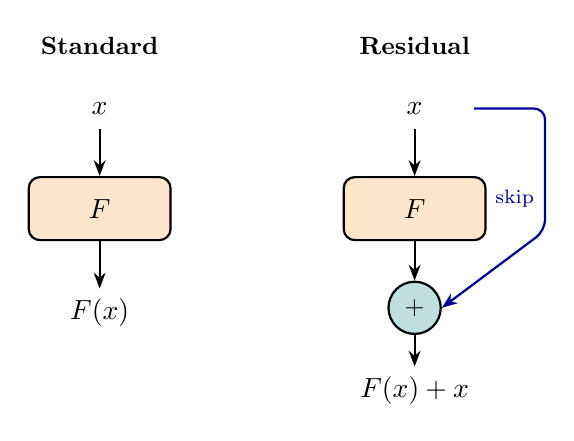
\begin{tikzpicture}[
    node distance=0.8cm,
    block/.style={rectangle, draw, rounded corners, minimum width=1.8cm, minimum height=0.8cm, fill=orange!20, thick},
    add/.style={circle, draw, minimum size=0.5cm, fill=teal!25, thick, font=\small},
    arrow/.style={-{Stealth[length=2mm]}, thick},
    skip/.style={-{Stealth[length=2mm]}, thick, rounded corners},
    label/.style={font=\scriptsize}
]

% Left side: Standard network (for comparison)
\node[font=\small\bfseries] at (-1.5, 1.8) {Standard};

\node[minimum width=1.5cm, minimum height=0.5cm] (in1) at (-1.5, 1.0) {$x$};
\node[block, below=0.6cm of in1] (l1a) {$F$};
\node[minimum width=1.5cm, minimum height=0.5cm, below=0.6cm of l1a] (out1) {$F(x)$};

\draw[arrow] (in1) -- (l1a);
\draw[arrow] (l1a) -- (out1);

% Right side: Residual block
\node[font=\small\bfseries] at (2.5, 1.8) {Residual};

\node[minimum width=1.5cm, minimum height=0.5cm] (in2) at (2.5, 1.0) {$x$};
\node[block, below=0.6cm of in2] (l1b) {$F$};
\node[add, below=0.5cm of l1b] (add) {$+$};
\node[minimum width=1.5cm, minimum height=0.5cm, below=0.4cm of add] (out2) {$F(x) + x$};

\draw[arrow] (in2) -- (l1b);
\draw[arrow] (l1b) -- (add);
\draw[arrow] (add) -- (out2);

% Skip connection
\draw[skip, blue!60!black] (in2.east) -- ++(0.9, 0) -- ++(0, -1.55) -- (add.east);

% Label the skip connection
\node[font=\scriptsize, blue!60!black, right] at (3.4, -0.15) {skip};

\end{tikzpicture}
\end{document}
